\documentclass[11pt,letterpaper,article,oneside]{memoir}
\usepackage[utf8]{inputenc}
\usepackage[T1]{fontenc}
\usepackage{microtype}
\usepackage[dvips]{graphicx}
\usepackage{xcolor}
\usepackage{times}

\usepackage{booktabs}

\usepackage{enumitem}
\setlist[description]{style=nextline}
\setlist[itemize]{nosep}

\usepackage[
breaklinks=true,colorlinks=true,
linkcolor=blue,urlcolor=blue,citecolor=blue,% PDF VIEW
%linkcolor=black,urlcolor=black,citecolor=black,% PRINT
bookmarks=true,bookmarksopenlevel=2]{hyperref}

\usepackage{geometry}
% PDF VIEW
% \geometry{total={210mm,297mm},
% left=25mm,right=25mm,%
% bindingoffset=0mm, top=25mm,bottom=25mm}
% PRINT
\geometry{total={210mm,297mm},
left=20mm,right=20mm,
bindingoffset=10mm, top=25mm,bottom=25mm}

\OnehalfSpacing
%\linespread{1.3}

%%% CHAPTER'S STYLE
%\chapterstyle{bianchi}
%\chapterstyle{ger}
%\chapterstyle{madsen}
%\chapterstyle{ell}

%%% STYLE OF SECTIONS, SUBSECTIONS, AND SUBSUBSECTIONS
\setsecheadstyle{\Large\bfseries\sffamily\raggedright}
\setsubsecheadstyle{\large\bfseries\sffamily\raggedright}
\setsubsubsecheadstyle{\bfseries\sffamily\raggedright}


%%% STYLE OF PAGES NUMBERING
%\pagestyle{companion}\nouppercaseheads 
%\pagestyle{headings}
%\pagestyle{Ruled}
\pagestyle{plain}
\makepagestyle{plain}
\makeevenfoot{plain}{\thepage}{}{}
\makeoddfoot{plain}{}{}{\thepage}
\makeevenhead{plain}{}{}{}
\makeoddhead{plain}{}{}{}

\maxsecnumdepth{subsection} % chapters, sections, and subsections are numbered
\maxtocdepth{subsection} % chapters, sections, and subsections are in the Table of Contents

\newcommand{\name}{PROGRAM\_NAME}
\newcommand{\version}{0.1}
\newcommand{\email}{eric.tytell@tufts.edu}

\renewcommand{\arraystretch}{1.2}

\setlength{\parindent}{0em}



%%%---%%%---%%%---%%%---%%%---%%%---%%%---%%%---%%%---%%%---%%%---%%%---%%%

\begin{document}

\thispagestyle{empty}

{%%%
%\sffamily
\centering
\Large

\vspace*{\fill}

{\huge
\name{} \version
}

{\LARGE
User manual \\
\vspace{2.5cm}
David Buckingham \\
Eric Tytell \\
Cassandra Donatelli \\
Margo \\
}
\vspace*{\fill}

}

\cleardoublepage

\tableofcontents*

\clearpage


\section{Copyright and License}

\name{}: a tool for collecting IMU measurements.
Copyright (C) 2017 Author(s)????????/

This program is free software: you can redistribute it and/or modify
it under the terms of the GNU General Public License as published by
the Free Software Foundation, either version 3 of the License, or
(at your option) any later version.

This program is distributed in the hope that it will be useful,
but WITHOUT ANY WARRANTY; without even the implied warranty of
MERCHANTABILITY or FITNESS FOR A PARTICULAR PURPOSE.  See the
GNU General Public License for more details.

You should have received a copy of the GNU General Public License
along with this program.  If not, see <http://www.gnu.org/licenses/>.

\section{Introduction}



%%%%%%%%%%%%%%%%%%%%%%%%%%%%%%%%%%%%%%%%%%%%%%
%             SECTION: HARDWARE              %
%%%%%%%%%%%%%%%%%%%%%%%%%%%%%%%%%%%%%%%%%%%%%%

\section{Hardware}

\name{} interconnects three pieses of computational hardware:
\begin{enumerate}
  \item a PC
  \item an Arduino
  \item between 1 and 3 Inertial Measurement Units (IMUs)
\end{enumerate}

\subsection{PC}
\name{} has been tested on PCs running Linux Mint 18 Sarah, OS X El Capitan
10.11, and Windows 10. It is expected to work with other versions of these
operating systems and with other Linux distributions.

\subsection{Arduino}
\name{} has been tested with an Arduino UNO. It may work on other
models having a 16MHz clock speed and sufficient storage.


\subsection{IMUs}
The mpu9250 by InvenSense is a nine-axis (gyroscope, accelerometer, compass)
motion tracking device.  For testing purposes, or if the added size and weight
are acceptable for your application, a mpu9250 mounted on a circuit-board can be
used with \name{}.

For applications requiring minimum package size and weight, it is possible to
wire the mpu9250 directly to the arduino. A separate manual, \textbf{name},
documents the procedure we have used to prepare the mpu9250 for use with
\name{}.


\subsection{Wiring the Arduino}
\label{sec:wiring}
Wire each IMU to the Arduino. It may be necessary to use a breadboard,
especially if multiple IMUs are used. Table \ref{tab:wiring} summarizes the
wiring process. The Arduino communicates with the IMUs using the Serial
Peripheral Interface bus (SPI) protocol. Each IMU needs a separate \emph{chip
select} line, but all IMUs share the other lines. Pins 8, 9, and 10 are used for
\emph{chip select} lines for up to three IMUs. Pin 11 is for data traveling from
the Arduino to the IMUs, i.e. Master-Out, Slave-In (MOSI). Pin 12 is for data
traveling from the IMUs to the Arduino, i.e. Master-In, Slave Out (MISO). Pin 13
is for a clock signal, used to regulate timing of the communication protocol. 

If using an optional trigger, wire it to Pin 4.

In addition, each IMU should be connected to 3.3V power (available on the
Arduino) and each IMU and the trigger should be connected to Ground.

Connect the arduino to the PC with a USB cable.

To ensure adequate power, especially if using multiple IMUs, it is recommended
to power the Arduino with an external power source instead of relying on the USB
port.



\begin{table}
\centering
\begin{tabular}{@{}*4l@{}}
\toprule
description & label & color & pin \\
\midrule 
IMU 1 chip select & NCS / CS & white & 8 \\
IMU 2 chip select & NCS / CS & white & 9 \\
IMU 3 chip select & NCS / CS & white & 10 \\
data from Arduino to IMU & MOSI / SDA & green & 11 \\
data from IMU to Arduino & MISO / SDO & blue & 12 \\
clock & SCL / CLK & yellow & 13 \\
power &  & red & 3.3V \\
ground &  & black & GND \\
trigger &  &  & 4 \\
\bottomrule
\end{tabular}
\label{tab:wiring}
\end{table}



%%%%%%%%%%%%%%%%%%%%%%%%%%%%%%%%%%%%%%%%%%%%%%
%          SECTION: INSTALLATION             %
%%%%%%%%%%%%%%%%%%%%%%%%%%%%%%%%%%%%%%%%%%%%%%

\section{Installation}

\name{} requires Python3.

We recommend using pip to install \name{}:
\url{https://pypi.python.org/pypi/pip}

\begin{verbatim}
# pip install --upgrade pip
# pip install \name
\end{verbatim}

Pip will automatically install any of the following dependencies if needed:
\begin{itemize}
\item h5py
\item numpy
\item pyqtgraph
\item pyserial
\item pyqt5
\end{itemize}


\subsection{Arduino code}

\subsubsection{Arduino IDE}
While there are many tools for installing program code onto the Arduino, we have
tested \name{} using the Arduino IDE.

The software can be downloaded from:
url{https://www.arduino.cc/en/Main/Software}

If you'r operating system has a package management system, it might be able
to install the Arduino IDE. For example, on Debian systems, use:
\begin{verbatim}
# apt-get install arduino-core
\end{verbatim}

\subsubsection{Install \name{} on the Arduino}
\label{sec:installarduinocode}

Install the file \verb|am_tx/am_tx.ino| on the Arduino.
This can be accomplished using the Arduino IDE graphical user interface.

Alternatively, using Arduino IDE version 1.5.0 or later,
the Arduino can be programmed directly from the command line:

\begin{verbatim}
# arduino --upload am_tx/am_tx.ino
\end{verbatim}

For more information about the Arduino command line interface, see:
\url{https://github.com/arduino/Arduino/blob/master/build/shared/manpage.adoc}

\section{Collecting data}

To begin collecting data, press the ``record'' button.
The PC will connect to the Arduino and instruct it to begin collecting data from
the IMUs at 200Hz. 


\subsection{Data buffer}

The ``data buffer length (\# samples)'' slider adjusts the size of the data
buffer... 


\subsection{Trigger}

Optionally, a trigger attached to the Arduino (Section \ref{sec:wiring}) can be
used to stop recording.  If the ``use trigger'' checkbox is not checked, the
trigger is ignored. Otherwise, if an ``active'' trigger is detected, recording
will stop, i.e., the same effect as pressing the ``stop'' button during
recording. If you attempt to begin recording while the ``use trigger'' checkbox
is checked and the trigger is ``active'', the recording end as soon as it starts
with zero data stored.

If the ``invert trigger'' checkbox is not checked, the trigger is considered
``active'' when the associated Arduino pin is set high. If the ``invert
trigger'' checkbox is checked, the trigger is considered ``active'' when the
associated Arduino pin is set low.

If there is nothing setting the current on the Arduino pin associated with the
trigger (i.e. if no trigger is connected), then the value of the pin is
undefined.  Thus, to ensure reliable behavior, the ``use trigger'' checkbox
should not be checked unless there is a trigger connected to the Arduino.

\begin{figure}[]
    \begin{center}
        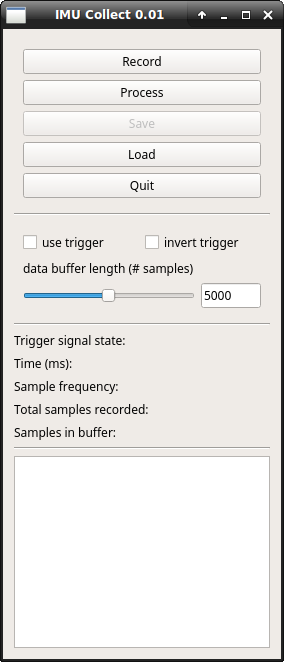
\includegraphics[width=.45\textwidth]{screenshot_0_imu}
    \end{center}
    \caption{Control panel} 
\end{figure}

\begin{figure}[]
    \begin{center}
        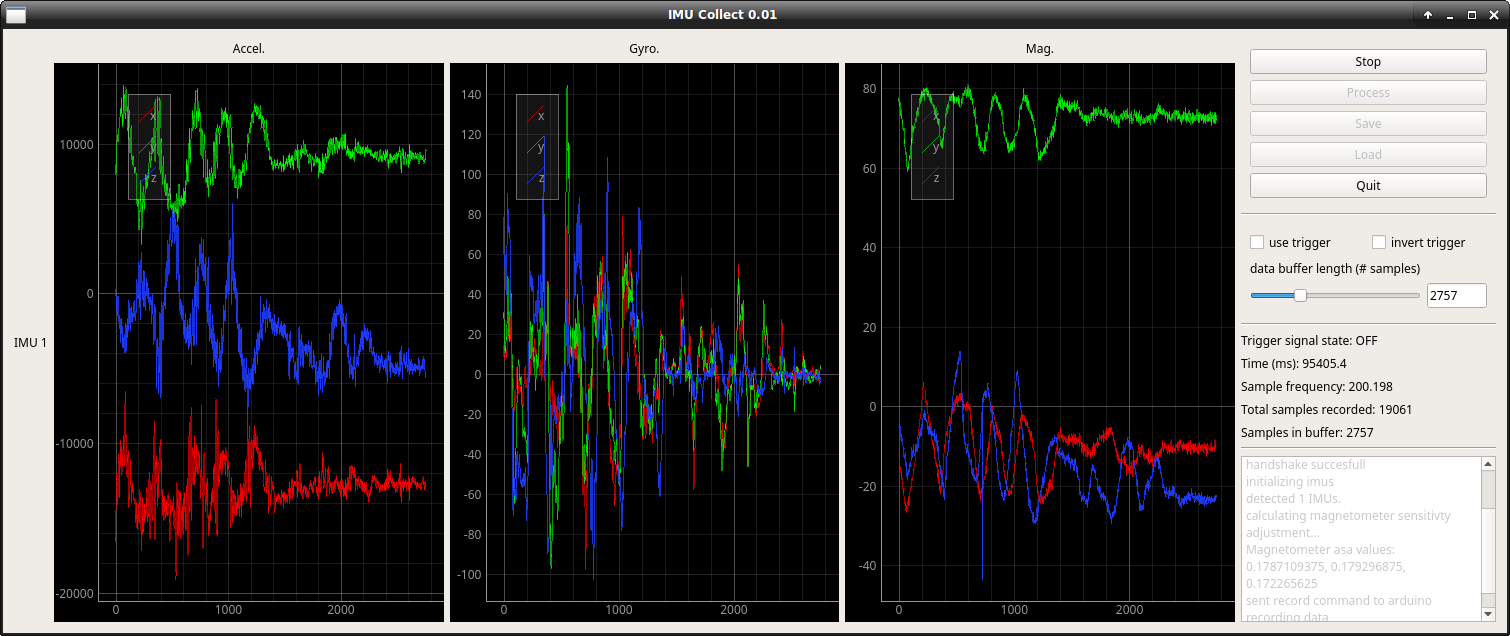
\includegraphics[width=.45\textwidth]{screenshot_1_imu}
    \end{center}
    \caption{Collecting data from a single IMU} 
\end{figure}





\section{Processing data}

\section{Saving and loading}
\label{sec:savingloading}

\subsection{.csv file format}
\label{sec:csv}
\name{} uses the CSV module in the Python Standard Library
with default formatting parameters:
\url{https://docs.python.org/3/library/csv.html}

\section{Settings}

\section{Troubleshooting}

\subsection{Error messages}

\begin{description}
\item[invalid csv file] The program attempted to read a .csv file (Section
\ref{sec:csv}), but the
format of the data in the file was not valid.

\item[invalid file type: ...]
\item[rx failed, no data read from serial]
\item[no Arduino found]
\item[failed to create connection]
\item[handshake failed]
\item[no connection, aborting]

\item[unable to determine number of IMUs, aborting] The program failed to
determine how many IMUs are attached to the Arduino. After the Arduino is
initialized, it attempts to determine the number of IMUs by sending a WHOAMI
request while signaling each of the three legal chip select pins (Section
\ref{sec:wiring}). It then sends a message to the PC reporting the number of
IMUs detected. This error is reported if the PC program sends a command to the
Arduino to initialize, but does not receive a message reporting the number of
IMUs detected. Make sure that any IMUs are correctly wired to the Arduino
(Section \ref{sec:wiring}) and that the correct code is installed on the Arduino
(Section \ref{sec:installarduinocode}), and try resetting the Arduino.

\item[no IMUs detected, aborting]

\item[ASA read failed, using 1 adjustment]

\item[Sample packet too short: ...]


\end{description}







%\bibliographystyle{unsrt}
%\bibliography{sample}

\end{document}

